%%Uncomment for lecture version
\documentclass[aspectratio=169]{beamer}
\usepackage{pgfpages}
%\setbeameroption{show notes on second screen=right}
%%Uncomment for handouts
%\documentclass[aspectratio=169, handout]{beamer}
\usepackage{./diegobeamer,mylistings}
\usepackage{datetime2}
\usepackage{tikz}
\usepackage{booktabs}
\usepackage{wrapstuff}
\usepackage{numprint}
\usepackage{wrapfig}
\usepackage{amsfonts}
\usepackage{mathpartir}
%\usepackage{marginnote}
% \usepackage{enumitem}
\usetikzlibrary{positioning,decorations.pathreplacing,fit, calc, backgrounds, matrix, shapes.multipart}
%\documentclass[aspectratio=169, notes=only]{beamer}
%\documentclass[notes]{beamer}       % print frame + notes
% Common settings for all lectures in this course
\usepackage{hyperref}
\usepackage{makecell}
\usepackage{array}
\usepackage{tcolorbox}
\renewcommand\UrlFont{\color{blue}\rmfamily}
\usepackage{amssymb}
\usepackage{amsmath}
\usepackage{numprint}
\usepackage{paralist}
\usepackage{stmaryrd}
\setbeamertemplate{footline}[frame number]
\usepackage{listings, xcolor}
\tikzset{hl/.style={
    set fill color=red!80!black!40,
    set border color=red!80!black,
  },
}
\usepackage{tcolorbox}

\tcbuselibrary{listings}
\tcbuselibrary{skins}

%\definecolor{verylightgray}{rgb}{.97,.97,.97}

\lstdefinelanguage{Solidity}{
	keywords=[1]{anonymous, assembly, assert, balance, break, call, callcode, case, catch, class, constant, continue, constructor, contract, debugger, default, delegatecall, delete, do, else, emit, event, experimental, export, external, false, finally, for, function, gas, if, implements, import, in, indexed, instanceof, interface, internal, is, length, library, log0, log1, log2, log3, log4, memory, calldata, modifier, new, payable, pragma, private, protected, public, pure, push, require, return, returns, revert, selfdestruct, send, solidity, storage, struct, suicide, super, switch, then, this, throw, transfer, true, try, typeof, using, value, view, while, with, addmod, ecrecover, keccak256, mulmod, ripemd160, sha256, sha3}, % generic keywords including crypto operations
	keywordstyle=[1]\color{blue}\bfseries,
	keywords=[2]{address, bool, byte, bytes, bytes1, bytes2, bytes3, bytes4, bytes5, bytes6, bytes7, bytes8, bytes9, bytes10, bytes11, bytes12, bytes13, bytes14, bytes15, bytes16, bytes17, bytes18, bytes19, bytes20, bytes21, bytes22, bytes23, bytes24, bytes25, bytes26, bytes27, bytes28, bytes29, bytes30, bytes31, bytes32, enum, int, int8, int16, int24, int32, int40, int48, int56, int64, int72, int80, int88, int96, int104, int112, int120, int128, int136, int144, int152, int160, int168, int176, int184, int192, int200, int208, int216, int224, int232, int240, int248, int256, mapping, string, uint, uint8, uint16, uint24, uint32, uint40, uint48, uint56, uint64, uint72, uint80, uint88, uint96, uint104, uint112, uint120, uint128, uint136, uint144, uint152, uint160, uint168, uint176, uint184, uint192, uint200, uint208, uint216, uint224, uint232, uint240, uint248, uint256, var, void, ether, finney, szabo, wei, days, hours, minutes, seconds, weeks, years},	% types; money and time units
	keywordstyle=[2]\color{teal}\bfseries,
	keywords=[3]{block, blockhash, coinbase, difficulty, gaslimit, number, timestamp, msg, data, gas, sender, sig, value, now, tx, gasprice, origin},	% environment variables
	keywordstyle=[3]\color{violet}\bfseries,
	identifierstyle=\color{black},
	sensitive=false,
	columns=flexible,
	comment=[l]{//},
	morecomment=[s]{/*}{*/},
	commentstyle=\color{gray}\ttfamily,
	stringstyle=\color{red}\ttfamily,
	morestring=[b]',
	morestring=[b]"
}

\lstdefinestyle{solidity_style}
{
	language=Solidity,
	%backgroundcolor=\color{verylightgray},
	extendedchars=true,
	basicstyle=\footnotesize\ttfamily,
	showstringspaces=false,
	showspaces=false,
	%numbers=left,
	numberstyle=\footnotesize,
	numbersep=9pt,
%    xleftmargin=5.0ex,	
    tabsize=2,
	breaklines=true,
	showtabs=false,
	captionpos=b,
	escapechar=!
}

\newtcblisting{soliditybox}[1][]{%
listing only,
listing options={language=Solidity, style=solidity_style, tabsize=2,escapeinside={(*@}{@*)}},
enhanced,
title=Solidity,
arc=1mm,
attach boxed title to top right = {xshift=-.5mm,yshift=-5.95mm},
boxed title style={size=small,arc=1mm, boxrule=0pt, sharp corners=downhill},
#1
}
\def\solidityinline{\lstinline[language=Solidity, style=solidity_style]}

\DeclareMathOperator{\dsum}{+}
\newcommand{\fromString}[1]{\ensuremath{\left\lceil#1\right\rceil}}
\newcommand{\toString}[1]{\ensuremath{\left\lfloor#1\right\rfloor}}
\newcommand{\update}[3]{
	\ensuremath{#1[#2\mapsto #3]}
}
\newcommand{\option}[1]{
	\ensuremath{#1}_\bot
}
\newcommand{\astack}[1]{\ensuremath{\mathit{sck}(#1)}}
\newcommand{\amemory}[1]{\ensuremath{\mathit{mem}(#1)}}
\newcommand{\astorage}[1]{\ensuremath{\mathit{sto}(#1)}}
\newcommand{\aaccount}[1]{\ensuremath{\mathit{acc}(#1)}}
\newcommand{\ustack}[2]{\ensuremath{\mathit{upSck}(#1,#2)}}
\newcommand{\umemory}[2]{\ensuremath{\mathit{upMem}(#1,#2)}}
\newcommand{\ustorage}[2]{\ensuremath{\mathit{upSto}(#1,#2)}}
\newcommand{\uaccount}[2]{\ensuremath{\mathit{upAcc}(#1,#2)}}
\newcommand{\Mod}[2]{#1~\mathrm{mod}~#2}

\newcommand{\tikzmark}[2][]{%
  \tikz[remember picture,overlay,baseline=-.5ex] \node[#1] (#2) {};%
}
% \drawBrace[xshift]{beginningNode}{endingNode}
% This command draws a brace between two tikzmarks, to their right,
% no matter which one is the rightmost, and includes 
% a node midway the brace, to write the comment.
% This command also creates a new node
% Whose name is the concat of the names of beginning and ending nodes.
\newcommand*{\drawBrace}[4][0pt]{%
    \node[draw=none, fit={(#2) (#3)}, inner sep=0pt] (rectg) {};%
    \draw [decoration={brace,amplitude=0.3em},decorate,very thick,red]%
      ([xshift=#1]rectg.north east) --%
      coordinate[right=.5em, midway] (#2#3)
      ([xshift=#1]rectg.south east);%
    \node[right=.4em of #2#3,align=left] (#2#3-comment) {#4};
    \draw (#2#3-comment.west) edge (#2#3);
}%
\def\lecturename{Computer Languages and Representations}
\def\lecturecode{ECM2418}
\def\coauthor{Achim D. Brucker}

\title{Isabelle/Solidity: A Tool for the Verification of Solidity Smart Contracts}
%\subtitle{Secure Smart Contracts with Isabelle/Solidity}
\author{ \textcolor{red}{\textbf{\underline{Asad Ahmed}}}, Diego Marmsoler}

\institute
{
  Department of Computer Science\\
  University of Exeter
}

\lecture[1]{Introduction}{introduction}
\date{\DTMdisplaydate{2025}{05}{04}{-1}}
\makeatletter
\def\blfootnote{\gdef\@thefnmark{}\@footnotetext}
\makeatother
\begin{document}
\begin{frame}[plain,noframenumbering]
\maketitle
\bigskip
\bigskip
%\begin{center}
%
\includegraphics[width=1.5 in]{logo.PNG}
%\end{center}
\begin{tikzpicture}[remember picture, overlay]
\node[yshift=-3cm] at (current page.center) 
{
    
\includegraphics[width=1.5 in]{logo2.PNG}
};
\end{tikzpicture}
\end{frame}

\frame{\tableofcontents}

\section{Introduction}
\frame{\tableofcontents[currentsection]}
%
%\subsection{Blockchain Technology}
%
%\begin{frame}{Blockchain Technology}
%\begin{itemize}
%\item A \textcolor{red}{database concept} which relies upon \textcolor{red}{decentralization }
%\end{itemize}
% \tikz \node at (0, 3) [font=\large,   minimum height=2.5em, minimum width = 3.25cm, inner sep=0pt, fill=blue!30] {Application Layer};
%\tikz \node [font=\normalsize, minimum height=2.5em, align = left] {Business logic for:\\[0.5pt]  Finance, Medical, Business, Agriculture etc.};\\
%\tikz \node [font=\large,  minimum height=2.5em, minimum width = 3.25cm, inner sep=0pt, fill=green!30 ] {Contract Layer};
%\tikz \node [font=\normalsize, minimum height=2.5em, align = left] {Programs in high-level languages to\\[0.5pt]  implement the business logic};\\
%\tikz \node [font=\large,  minimum height=2.5em, minimum width = 3.25cm, inner sep=0pt, fill=blue!30] {Consensus layer};
%\tikz \node [font=\normalsize, minimum height=2.5em, align = left] {Set of rules agreed upon to add a new block,\\[0.5pt] such as  Proof of Work (PoW)};\\
%\tikz \node [font=\large,  minimum height=2.5em, minimum width = 3.25cm, inner sep=0pt, fill=blue!30] {Network Layer};
%\tikz \node [font=\normalsize, minimum height=2.5em, align = left] {Handles the communication between nodes};\\
%\tikz \node [font=\large,  minimum height=2.5em, minimum width = 3.25cm, inner sep=0pt, fill=blue!30] {Data Layer};
%\tikz \node [font=\normalsize, minimum height=2.5em, align = left] {Data transactions, Blocks, Cryptography};\\
%\begin{exampleblock}{}
%  {\large \begin{center}Smart contracts provide an interface to real-world applications\end{center}}
%\end{exampleblock}
%\end{frame}
%
\subsection{Smart Contracts}
\begin{frame}{Smart Contracts}

 \begin{itemize}

\item \textcolor{red}{Programs} that \textcolor{red}{automate the transactions} in a Blockchain
\begin{itemize}
\item[--] \textcolor{red}{Executes when agreed upon conditions are met}
\end{itemize}
\item Key feature is: \textcolor{red}{once deployed cannot be modified}
\item \textcolor{red}{Solidity} is the most \textcolor{red}{popular high-level language} to write smart contracts (\textcolor{red}{90\%} of all smart contracts are developed using Solidity)
\item \textcolor{red}{Bugs} may lead to \textcolor{red}{huge financial losses}
\begin{itemize}
\item[--] (\textcolor{red}{DAO}) smart contract was manipulated to steal around \textcolor{red}{2 Million USD worth Ether}
\end{itemize}
\end{itemize}
\end{frame}
%


%
\subsection{Isabelle/Solidity Implementation}
\begin{frame}{Isabelle/Solidity Implementation}
\begin{figure}[t]
    \centering
    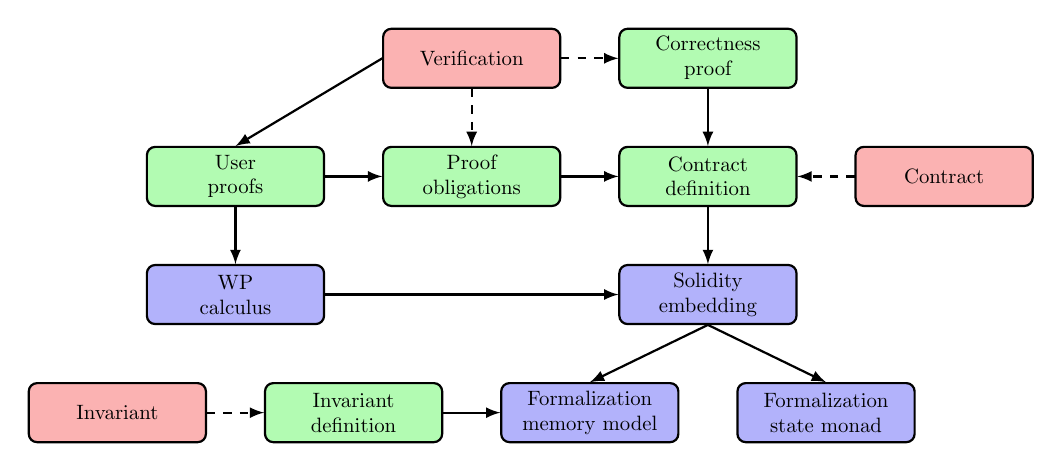
\begin{tikzpicture}[%
        thick,scale=0.75, every node/.style={scale=0.75},
        basic/.style ={rounded corners=3pt, draw, minimum width=3cm, minimum height=1cm, align=center},
        theory/.style={basic, fill=blue!95!black!30},
        temp/.style={basic, fill=green!95!black!30},
        feature/.style={basic, fill=red!95!black!30},
        dep/.style={-latex},
        gen/.style={-latex,dashed}
        ]
        \node[feature] (ver) at (0,0) {Verification};
        \node[temp] (obl) at (0,-2) {Proof \\ obligations};
        \node[temp] (usr) at (-4,-2) {User \\ proofs};
        \node[temp] (cor) at (4,0) {Correctness \\ proof};
        \node[temp] (cnt) at (4,-2) {Contract \\ definition};
        \node[feature] (spc) at (8,-2) {Contract};
        \node[theory] (wpc) at (-4,-4) {WP \\ calculus};
        \node[theory] (lan) at (4,-4) {Solidity \\ embedding};
        \node[feature] (isc) at (-6,-6) {Invariant};
        \node[temp] (idf) at (-2,-6) {Invariant \\ definition};
        \node[theory] (fmm) at (2,-6) {Formalization \\ memory model};
        \node[theory] (fsm) at (6,-6) {Formalization \\ state monad};
        \draw[dep] (ver.west) -- (usr.north);
        \draw[gen] (ver.south) -- (obl.north);
        \draw[gen] (ver.east) -- (cor.west);
        \draw[dep] (cor.south) -- (cnt.north);
        \draw[gen] (spc.west) -- (cnt.east);
        \draw[dep] (usr.south) -- (wpc.north);
        \draw[dep] (usr.east) -- (obl.west);
        \draw[dep] (obl.east) -- (cnt.west);
        \draw[dep] (cnt.south) -- (lan.north);
        \draw[dep] (wpc.east) -- (lan.west);
        \draw[dep] (lan.south) -- (fsm.north);
        \draw[dep] (lan.south) -- (fmm.north);
        \draw[dep] (idf.east) -- (fmm.west);
        \draw[gen] (isc.east) -- (idf.west);
    \end{tikzpicture}
    \caption{Isabelle/Solidity: theories (blue), commands (red), and generated artefacts (green). \label{fig:approach}}
\end{figure}
\end{frame}



\section{Case Study}
%\frame{\tableofcontents[currentsection]}

%\begin{frame}{Bank}
%\begin{itemize}
%\item Keeps an internal record of funds transferred by its customers.
%\item This record is increased whenever a customer transfers additional funds 
%\item When customer withdraws all its recorded
%funds are returned and its internal record reset to 0.
%\end{itemize}
\subsection{Casino Smart Contract}
%
\begin{frame}{Casino}
\begin{itemize}

\item The casino contract implements a betting game based on guessing  the outcome of coin-tossing.
\begin{itemize}
\item[--] \textcolor{red}{Operator} creates a game by placing \textcolor{red}{HEAD/TAIL} as a \textcolor{red}{ secret} against an \textcolor{red}{ amount} \textcolor{blue}{ (pot)}
\item[--] \textcolor{red}{Player} places a \textcolor{blue}{ bet} by \textcolor{red}{guessing} the secret 
\item[--] \textcolor{red}{Operator} decides the bet using \textcolor{red}{guess} and \textcolor{red}{secret}
\item[--] If player wins \textcolor{blue}{ bet} is doubled else \textcolor{blue}{bet} is transferred to \textcolor{blue}{pot}
\end{itemize}
\item \textcolor{red}{Solidity  implementation} utilizes many advanced features of Solidity Language, e.g.,:
\begin{itemize}
\item[--] \textcolor{red}{Types, Functions, Modifiers }
\end{itemize}
%\item \textcolor{red}{Verification Challenges:} Specification, Preconditions, postconditions, Invariants
\end{itemize}
\end{frame}
%%
%%
\section{Isabelle/Solidity}
\subsection{Specification}
\subsubsection{Types \& Variable(s) }
\begin{frame}{Types \& Variable(s)}
\begin{columns}
\begin{column}{0.5\textwidth}
  \begin{itemize}

\item \textcolor{blue}{contract} command followed by the \textcolor{green}{names of contract}, \textcolor{green}{storage variables} and \textcolor{green}{constructor}
\item Supports formal specification of Solidity Types: \textcolor{green}{value types, reference types, mappings and customized types}  
%\item \textcolor{green}{constructor payable where} keywords combination to specify body of constructor 
%\begin{itemize}
%\item[--] \textcolor{green}{payable} is a function modifier allows the contract receive \textit{ethers} 
%\item[--] As casino does not have constructor thus \textcolor{blue}{$<$skip$>$}
%\end{itemize}

\item \textcolor{green}{payable} is a function modifier allows the contract receive \textit{ethers} 
\end{itemize}
\end{column}
\begin{column}{0.5\textwidth}  %%<--- here
    \begin{center}
     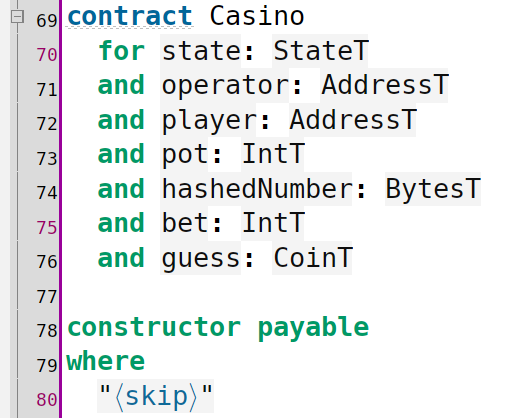
\includegraphics[width=0.75\textwidth]{contract_storage.png}
     \end{center}
\end{column}
\end{columns}
\end{frame}
%%
\subsubsection{Function(s)}
\begin{frame}{Function(s)}
\begin{columns}
\begin{column}{0.40\textwidth}
  \begin{itemize}
\item \textcolor{green}{emethod} keyword followed by the \textcolor{green}{name of the function, modifier(s), parameter(s) and body of the function}
\item Supports stack \textcolor{green}{(param)}, memory \textcolor{green}{(memory)} and calldata \textcolor{green}{(calldata)} types of store  variables
\item \textcolor{green}{where "do\{\}"} formally specifies body of the functions  

\end{itemize}
\end{column}
\begin{column}{0.60\textwidth}  %%<--- here
    \begin{center}
     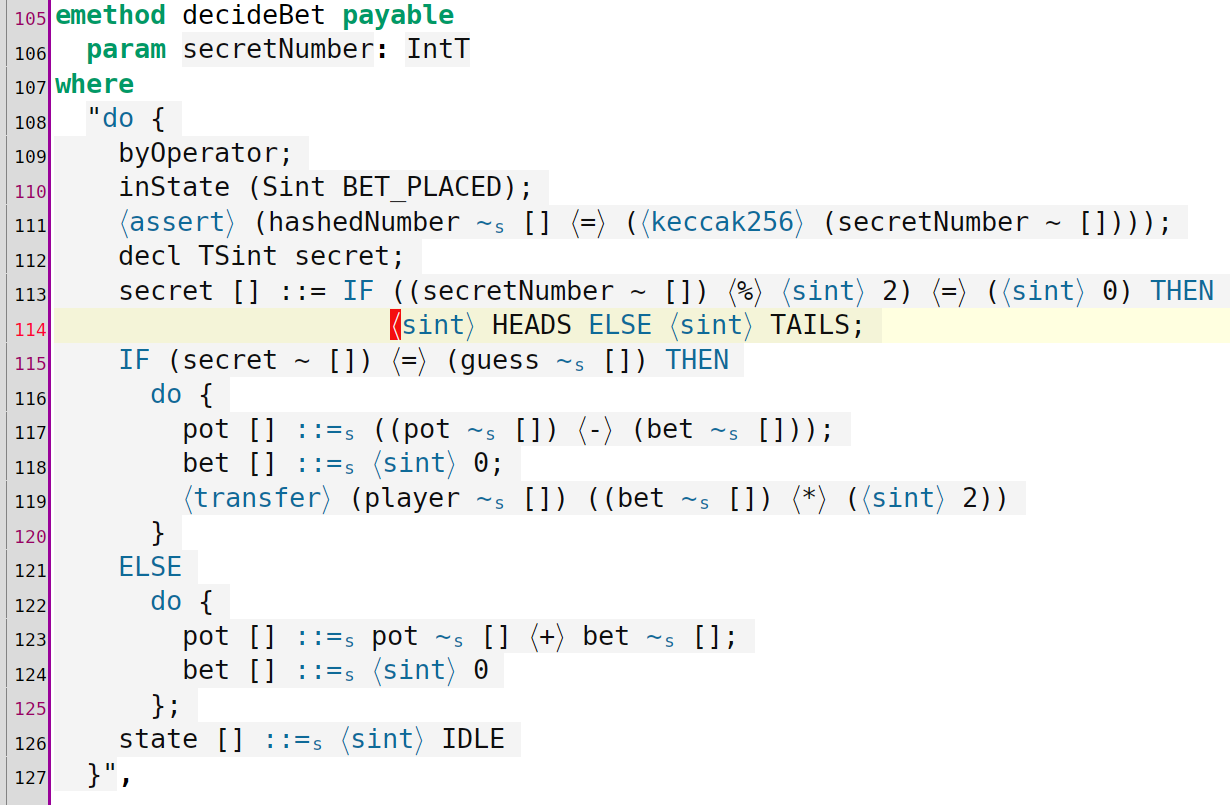
\includegraphics[width=\textwidth]{method_contract.png}
     \end{center}
\end{column}
\end{columns}
%\begin{itemize}
%
%\item \textcolor{blue}{contract} keyword followed by the contract name
%\item \textcolor{green}{for...and} keyword followed by the contract storage variables
%
%\end{itemize}
%	\begin{center}
%		\fbox{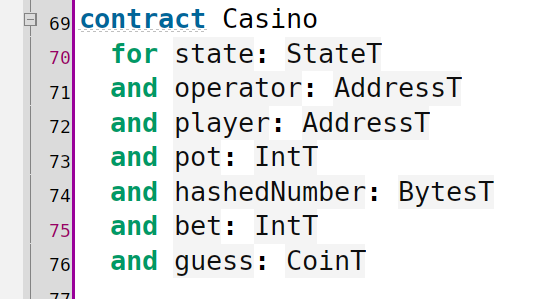
\includegraphics[width = 0.5\textwidth]{casino_storage.png}}
%	\end{center}
\end{frame}
\subsubsection{Invariant}
\begin{frame}{Invariant}
\begin{Example}{}{}
Assume that we want to ensure our contract has always enough funds to cover the payout of players.
  More formally, we want to ensure that, whenever the game is in the \texttt{BET\_PLACED} state, the contract's internal balance satisfies:
	\begin{equation}
	  \textrm{\textit{pot\_balance(s, b}})=\textrm{\textit{b}} \ge \textrm{\textit{s}}(\textrm{\textit{``pot"}}) + \textrm{\textit{s}}(\textrm{\textit{``bet"}})~\wedge~\textrm{\textit{s}} \textrm{\textit{(``bet")}} \leq \textrm{\textit{s}}\textrm{\textit{(``pot")}}
	\end{equation}
  and if it is not in \texttt{BET\_PLACED}, then 
  \begin{equation}
		\textrm{\textit{pot\_balance(s, b)}} =\textrm{\textit{b}} \ge \textrm{\textit{pot}} 
  \end{equation}
%
The corresponding specification in Isabelle/Solidity is:
		\begin{center}\vspace{-2mm}
		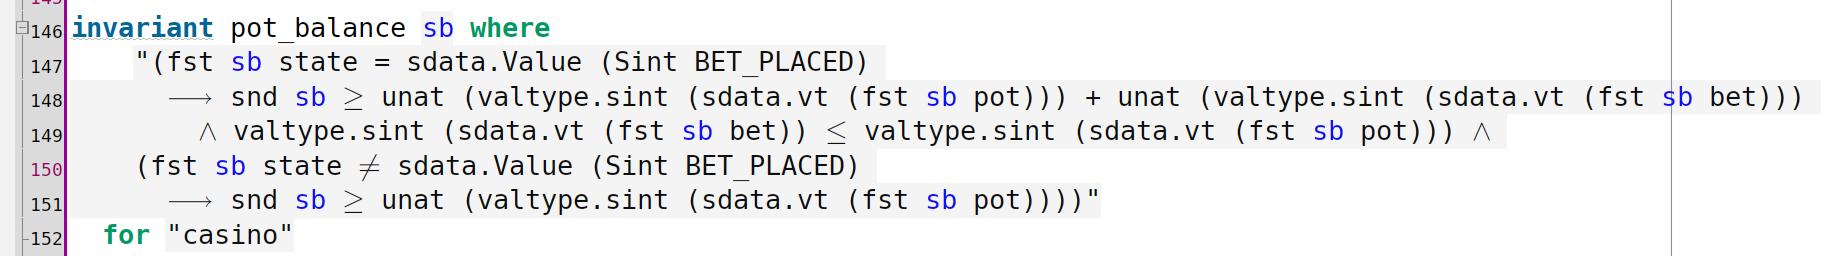
\includegraphics[width=.95\textwidth]{inv_spec.png}
	\end{center}\vspace{-2mm}
\end{Example}
\end{frame}
%
%%%%
\subsection{Verification}
\begin{frame}{Verification}
\begin{columns}
\begin{column}{0.50\textwidth}
  \begin{itemize}
\item \textcolor{blue}{verification} command is followed by:
\begin{itemize}
\item[--] invariant over contract balance and store: \texttt{pot\_balance} 
\item[--] Postcondition for the constructor: \texttt{K(K(K True))}
\item[--] methods and corresponding postconditions 
\item[--] name of the smart contract: \texttt{casino}
\end{itemize}
\item \textcolor{blue}{verification} attempts to generate \textcolor{green}{correctness theorem} and results in \textcolor{green}{proof obligations}
\end{itemize}
\end{column}
\begin{column}{0.50\textwidth}  %%<--- here
  \begin{center}
     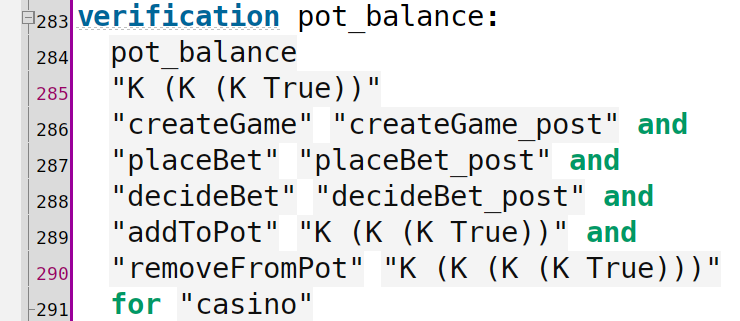
\includegraphics[width=\textwidth, height=3cm, keepaspectratio]{ver_conract}
     \end{center}
\end{column}
\end{columns}
\end{frame}


%%
\begin{frame}{Automatic Verification}
\begin{itemize}
\item To automatically discharge the proof obligations, tool has verification condition generator based on weakest precondition calculus
\item Automatic verification using \texttt{vcg} has been shown for \texttt{creatGame} method
\begin{center}\vspace{2mm}
		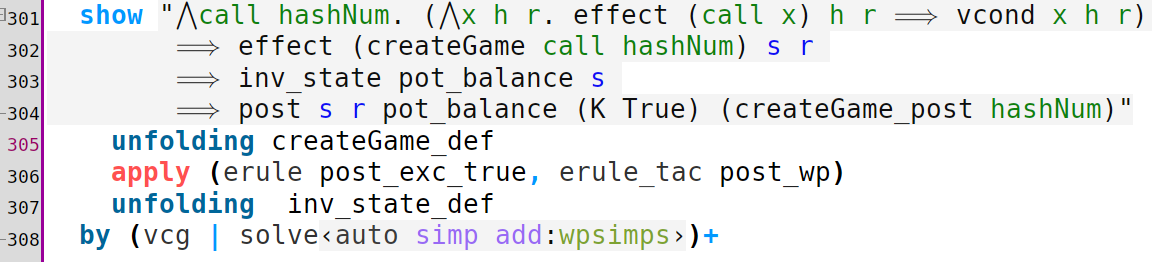
\includegraphics[width=.95\textwidth]{inv_contract.png}
	\end{center}\vspace{2mm}
\end{itemize}
\end{frame}
%
\section{Conclusion}
\frame{\tableofcontents[currentsection]}

\begin{frame}{Conclusion}
Summary
\begin{itemize}
	\item Proposed \textcolor{red}{Isabelle/Solidity}, a tool for the \textcolor{red}{formal specification and verification
	of Solidity smart contracts} within \textcolor{red}{Isabelle theorem prover}
	\item Tool facilitates \textcolor{red}{Solidity types, types of stores, functions, modifiers, expressions and statements} to facilitate formal specification of smart contracts
	\item Tool supports verification of smart contract \textcolor{red}{invariants and postconditions}
		\item Tool facilitates automatic  verification using \textcolor{red}{verification condition generator}
	\item  \textcolor{red}{casino smart contract} and \textcolor{red}{corresponding invariant} is formally specified and verified as a case study.

\end{itemize}
\bigskip

Future Work: 
\begin{itemize}
	\item Some advanced features such as \textcolor{red}{inheritance}
\end{itemize}
\end{frame}
%%%%%%%%%%%
\begin{frame}{}
	\begin{center}
{\fontsize{40}{50}\selectfont Thank You!}\\
\vspace{0.5in}
{\fontsize{30}{40}\selectfont \textcolor{white}{\colorbox{blue}{Q\&A}}}\\
\end{center}
\end{frame}
%%%%%%%%%
%


\end{document}